\scanpage{128}
\mspage{2}
% archive sheet number: 127
\unsure{où}
\diagram{\begin{tikzcd}[ampersand replacement=\&,execute at end picture={
\node[anchor=east] at ([xshift=-5pt]current bounding box.west) {$\deleted{\unsure{F|P}}\unsure{\Phi|\mathcal F|F}_\alpha(f)=\Bigl\{$};
\node[anchor=west] at ([xshift=5pt]current bounding box.east) {$\Bigr\}$};}]
X \arrow[r,"\deleted{\unsure{\Sigma_\alpha|I_\alpha}}i_\alpha(f)"] \& X_\alpha(f) \arrow[r,Rightarrow,"p_\alpha(f)"] \& Y
\end{tikzcd}}
\[\tag*{1.9.}\]
avec $p_\alpha(f)\deleted{\Sigma_\alpha}i_\alpha(f)=f$. La fonctorialité de 1.4. et 1.5., ou celle de $\Phi_\alpha$ i.e. de 1.9., s'exprime par le fait que tout \deleted{diagramme}\inserted{carré} commutatif
\diagram{\begin{tikzcd}[ampersand replacement=\&]
X \arrow[r,phantom,"\unsure{\overset{f}{\longrightarrow}|\overset{f}{\longleftrightarrow}}"] \arrow[d,"u_X"'] \& Y \arrow[d,"u_Y"] \\
X' \arrow[r,"f'"'] \& Y'
\end{tikzcd}}
\[\tag*{1.10.}\]
dans $M$, interprété comme flèche $u=(u_X,u_Y)$ de $f$ dans $f'$ dans $\underline{\mathrm{Fl}}(M)$, donne \unsure{naissance} à un double carré commutatif
\diagram{\begin{tikzcd}[ampersand replacement=\&]
X \arrow[r,Rightarrow,"\deleted{\Sigma_\alpha}i_\alpha(f)"] \arrow[d,"u_X"'] \& \deleted{\unsure{\Sigma_\alpha|Z_\alpha}}X_\alpha(f) \arrow[r,"p_\alpha(f)"] \arrow[d,"X_\alpha(u)"] \& Y \arrow[d,"u_Y"] \\
X' \arrow[r,Rightarrow,"\deleted{\Sigma_\alpha}i_\alpha(f')"'] \& X_\alpha(f') \arrow[r,"p_\alpha(f')"'] \& Y'
\end{tikzcd}}
\[\tag*{1.11.}\]
.

\uline{NB} Quand on voudra expliciter la dépendance de \unsure{ces|mes} constructions p.r. à $C_0$, on écrira
% Original horizontal order retained with the handwritten transposition stroke reproduced.
\figure{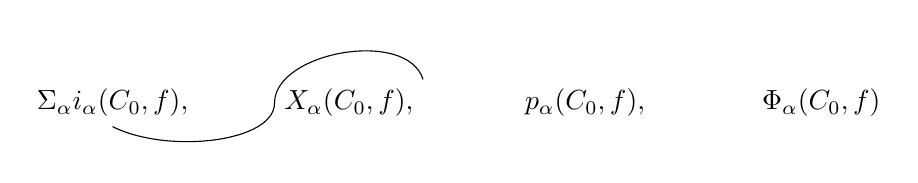
\begin{tikzpicture}
\node (a) at (0,0) {$\deleted{\Sigma_\alpha}i_\alpha(C_0,f),$};
\node (b) at (3,0) {$X_\alpha(C_0,f),$};
\node (c) at (6,0) {$p_\alpha(C_0,f),$};
\node (d) at (9,0) {$\Phi_\alpha(C_0,f)$};
\draw (a.south) .. controls +(0.7,-0.35) and +(0,-0.5) .. (b.west) .. controls +(0,0.65) and +(-0.2,0.65) .. (b.north east);
\end{tikzpicture}}
ou
\figure{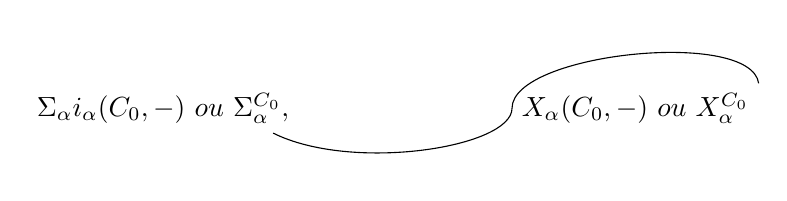
\begin{tikzpicture}
\node (a) at (0,0) {$\deleted{\Sigma_\alpha}i_\alpha(C_0,-)\ \text{ou}\ \Sigma_\alpha^{C_0},$};
\node (b) at (6,0) {$X_\alpha(C_0,-)\ \text{ou}\ X_\alpha^{C_0}$};
\draw ([xshift=1.4cm]a.south) .. controls +(1,-0.5) and +(0,-0.5) .. (b.west) .. controls +(0,0.7) and +(-0.1,0.7) .. (b.north east);
\end{tikzpicture}}
au lieu de $\deleted{\Sigma_\alpha}i_\alpha(f)\ \ldots\ ,\ \deleted{\Sigma_\alpha}i_\alpha,\ \ldots$ .

Voici les propriétés essentielles du système inductif ordinal des $\deleted{\Sigma_\alpha}X_\alpha(f)$ ou $\Phi_\alpha(f)$.
